\chapter{LEARNING SHARED STRUCTURE FROM HETEROGENEOUS DATA}
\label{ch:latent-bandits}

\aigen{\emph{This chapter is based on joint work with Chinmaya Kausik and Ambuj Tewari \citep{kausik2024leveragingofflinedatalinear}: Chinmaya Kausik, Kevin Tan, and Ambuj Tewari, ``Leveraging Offline Data in Linear Latent Contextual Bandits, in Proceedings of the 41st International Conference on Machine Learning (ICML), PMLR 235:23476--23516, 2024.}}

\todoresolve{CHECK WHETHER SECTION 3.7 (DE FINETTI THEOREM FOR STATELESS DECISION PROCESSES) SHOULD REMAIN IN THE MAIN CHAPTER OR MOVE TO APPENDIX B FOR PACING.}

\section{Introduction}

Many sequential-decision making problems can be effectively modeled using the bandit framework. This can span domains as diverse as healthcare \cite{lu2021bandit}, randomized clinical trials \cite{press2009rct}, search and recommendation \cite{Li_2010}, distributed networks \cite{kar2011banditnetworks}, and portfolio design \cite{brochu2011portfolio}. There is often a wealth of offline data in such domains, which has led to a growing interest in using offline data to accelerate online learning. However, there often also exist unobserved contexts in the population that influence the distribution of rewards, making it non-trivial to leverage offline data. In \citet{hong2020latent}, it is shown that this uncertainty can be modeled by a \textit{latent bandit} (or mixture of bandits). This is a bandit where an unobserved latent state determines the reward model for the trajectory. For example, a patient's underlying genetic conditions in healthcare and a user's tastes in recommendation systems are both examples of latent states in sequential decision making. Typically, these latent states are less complex than the actual models underlying users or patients, making it valuable to reduce the online task to learning the latent state \cite{hong2020latent, hong2022thompsonsamplingmixtureprior}.

 
%However, the extent of the generality of this framework is unclear. Given a general decision process, how strong do the conditions need to be to make it a latent bandit? To answer this, we turn to de Finetti's celebrated theorem, which says that exchangeable sequences of Bernoulli random variables are mixtures of sequences of i.i.d. Bernoulli random variables. This has also been extended to larger classes of stochastic processes \cknote{cite}, but not to decision processes. Inspired by such work, we define a general stateless decision process, and consider a weak notion of exchangeability as well as a natural coherence condition. We show that in the spirit of de Finetti's theorem, \textit{any} coherent and exchangeable stateless decision process is a latent bandit. \cknote{laying out the space of latent bandits}
The latent bandit framework therefore has high practical value, and efficient principled algorithms are needed for using offline data to speed up online learning. Using traditional bandit algorithms in this setting does not leverage the offline data that is often available to the agent. Naturally, one also cannot treat the offline data as coming from a single bandit. For example, different user tastes or different underlying genetic conditions require modeling the offline data as coming from a latent bandit. So, we have to develop algorithms \textit{specific} to the latent bandit setting that leverage the offline data to improve online performance. 

 
We note that in bandit literature, it is common to impose a structure on bandit rewards when designing algorithms, the most popular one being a linear structure \cite{Li_2010, abbasi2011improved}. In this light, we study a linear contextual bandit setting where each user has its own high-dimensional reward parameter, but reward parameters across users lie in a low-rank subspace. This is a \textit{linear latent contextual bandit}\footnote{This can also be thought of as a continuous mixture of bandits.}, and is much more general than existing models that restrict themselves to finitely many latent states \cite{,hong2020latent, hong2022thompsonsamplingmixtureprior}. We design a two-pronged algorithm to tackle this setting. First, we provide a method to approximate the low-dimensional subspace spanned by latent states from an offline dataset of unlabeled trajectories collected under some behavior policy $\pi_b$. This is non-trivial since the trajectories are unlabeled, and standard unsupervised learning methods fail. Second, we use this subspace to speed up online learning. However, since the subspace is only learnt \textit{approximately,} we also tackle the non-trivial task of accounting for the uncertainty in the subspace. We design two methods for the latter, facing a trade-off between computational tractability and tightness of guarantees. Experiments show the efficacy of our methods. 

While latent bandits have thus shown to be a powerful and tractable framework for accounting for uncertainty in reward models, the extent of their {\em generality} is unclear. Are there other stateless decision processes that generalize over latent bandits? We end by theoretically demonstrating that under very reasonable assumptions, the answer is no. We show a de Finetti theorem for decision processes, demonstrating that \textit{every} "coherent" and "exchangeable" stateless (contextual) decision process is a latent (contextual) bandit. With this in mind, we outline our contributions below:
 
\begin{itemize}  
    \item \textbf{Offline method:} We present \aigen{Algorithm~\ref{alg:sold}}, a novel offline method for learning low-dimensional subspaces of reward parameters with guarantees, inspired by the novel spectral methods in \citet{kausik2023learning}.
    \item \textbf{Tight online algorithm:} We present \aigen{Algorithm~\ref{alg:local-ucb}}, an online algorithm leveraging the subspace estimated offline to sharpen optimism, achieving $\tilde O(\min(d_A\sqrt{T}, d_K\sqrt{T}(1+\sqrt{d_AT/d_KN})))$ regret.
    \item \textbf{Lower Bound:} We establish a matching lower bound showing that \aigen{Algorithm~\ref{alg:local-ucb}} is minimax optimal. To the best of our knowledge, this is the first lower bound in a hybrid (offline-online) sequential decision-making setting.
    \item \textbf{Tractable online algorithm:} Finally, we present \aigen{Algorithm~\ref{alg:proball-ucb}}, a practical and computationally efficient online algorithm with a slightly looser regret guarantee. This also illustrates a general algorithmic idea for integrating offline subspace estimation into optimistic algorithms.
    \item \textbf{Experiments:} We establish the efficacy of our algorithms outlined above through a simulation study and a demonstration on a real recommendation problem with the MovieLens-1M \cite{movielens} dataset.
    \item \textbf{Theoretical generality:} We are the first, to our knowledge, to prove a de Finetti theorem for decision processes. This establishes the generality of the latent bandit model.
\end{itemize}

\textbf{Related work.} There are three main threads of related work.
 
\begin{itemize}  
\item \textbf{Latent Bandits.} The line of work most relevant to us has been on latent bandits. The work of \citet{hong2020latent, hong2022thompsonsamplingmixtureprior} studies the latent bandit problem under finitely many states. However, they black-box the offline step and do not provide end-to-end guarantees, and their ideas do not extend to infinitely many states. Our work seeks to provide end-to-end guarantees for both the offline and online component under infinitely many latent states.
\item \textbf{Meta learning, multi-task learning and mixture learning.} A long line of work studies learning with multiple underlying tasks or models. For example, the work of \citet{vempala2004spectral, kakade2020meta, anandkumar2014tensordecompositionslearninglatent, tripuraneni2022provablemetalearninglinearrepresentations} study learning under latent variable or multi-task models in a supervised setting. The work of \citet{kausik2023learning, poor2022mixdyn} extend some of these ideas to unsupervised but purely offline learning in a time-series setting. On the other hand, work like \citet{yang2022nearlyminimaxalgorithmslinear, cella2022metarepresentationlearningcontextual} instead focuses on the purely online setting of learning the low-rank structure while simultaneously interacting with multiple finitely many bandit instances. Finally, \citet{zhou2024federatedofflinereinforcementlearning, lu2021powermultitaskrepresentationlearning} work with multiple underlying models in MDPs but in a purely offline and generative model setting respectively. Unlike these papers, we crucially combine the offline and online settings for sequential data and study the problem of using offline data to accelerate online learning in bandits.
% \item \textbf{Multi-task bandits and RL.} \cite{yang2022nearlyminimaxalgorithmslinear} consider the case where there are $T$ linear bandits, each with dimension $d$, and where these $T$ bandit tasks share a common $k \ll d$ dimensional representation. Their paper works in a purely online setting where multiple but finitely many bandit instances are being interacted with. In contrast, despite a shared latent structure between bandit problems, we have to leverage a wealth of offline data across a continuum of bandit instances. Offline federated or multi-task RL \citep{zhou2024federatedofflinereinforcementlearning, lu2021powermultitaskrepresentationlearning}, on the other hand, seeks to learn a task-dependent policy given labeled data from a finite set of task MDPs. This is in contrast to our setting, where we have unlabeled logged bandit data from ture of bandits. 
\item \textbf{Hybrid (offline-online) RL.} Work in hybrid RL studies the use of offline data to accelerate online RL, first proposed by \citet{song2023hybrid}, with extensions to linear MDPs by \citet{wagenmaker2023leveraging, tan2024hybridreinforcementlearningbreaks}. \citet{cai2024transferlearningcontextualmultiarmed} studies the same problem for contextual bandits. However, all work so far assumes that the offline data is generated by a single model, and does not account for latent states. Our work explores a hybrid offline-online setting while also accounting for the offline data being generated by multiple underlying models.
\end{itemize}
 
% strict assumptions on task covariance matrix, if you treat trajectory as a task, the dimension grows in offline horizon length, blowing up the estimation guarantee. to avoid this, one needs to develop methods specifically for logged bandit data. another option is to treat every s,a,r pair as a task. this is invalid because the s,a,r pairs are not iid in our setting. 

% There is a line of work in offline RL with multiple sources of offline data that come from different models. \cite{shi2023provablyefficientofflinereinforcement} consider a setting where they consider mutliple sources of offline data that come from different MDPs, where the rewards in each source have the same
% expectation as the rewards in a target task they wish to solve. \cite{kausik2024confounded} propose a variant of RL in the presence of unobserved confounding that seeks to learn a single policy that performs well on a set of MDPs, given a dataset of unlabeled data from the MDPs. This corresponds to an offline version of the latent MDP framework of \cite{kwon2021rllatentmdpsregret} that is solved by learning a mixture of MDPs \citep{kausik2023learning} before applying offline RL. Offline federated or multi-task RL \citep{zhou2024federatedofflinereinforcementlearning, lu2021powermultitaskrepresentationlearning}, on the other hand, seeks to learn a task-dependent policy given data from a set of task MDPs. 

\section{Linear Bandits With Latent Structure}

We will first introduce latent contextual bandits, and then specialize to our linear model later in this section. A latent contextual bandit is a decision process with contexts $\gX$, actions $\gA$ and an random latent state $\theta$ that is sampled independently at the beginning of each trajectory. Given a sequence of contexts and actions, the rewards at all steps are independent \textit{conditioned} on $\theta$, and depend on the latent state $\theta$, the context and the action. Since we often have access to an offline dataset of trajectories coming from different kinds of users or patients, it is important to account for a changing latent state $\theta$ between trajectories.

 
As we will see in Section~\ref{sec:de-finetti}, latent bandits are a powerful and general framework for encoding uncertainty in reward models. However, this generality is both a blessing and a curse. It is hard to design concrete algorithms without further assumptions on the structure and effect of the latent state $\theta$. We therefore focus on a linear structure here. We consider the natural generalization of the linear contextual bandit to the latent bandit setting, where we impose a linear structure on the effect of low-dimensional latent states. We further justify this by noting that in most application domains, it is reasonable to assume that a parsimonious, low-dimensional latent state affects the reward distribution. This motivates the following definition.

\begin{definition}
    A \textit{linear latent contextual bandit} is a linear bandit equipped with a feature map for context-action pairs $\phi: \gX \times \gA \to \Real^{d_A}$, a latent random variable $\btheta \in \Real^{d_K}$ with distribution $\gD_\theta$ and a map $\BU_\star: \Real^{d_K} \to \Real^{d_A}$ such that for any $H$ and context-action sequence $((x_1, a_1), \dots (x_H, a_H))$, the rewards $(Y_1, \dots Y_H)$ are independent conditioned on $\btheta$. Moreover, $Y_h \mid \btheta \sim \phi(x_h,a_h)^\top \bbeta + \epsilon$, where $\epsilon$ is subgaussian noise independent of all actions and all other observations, and $\bbeta = \BU_\star \btheta$. 
    \label{defn:latent-linear-bandit}
\end{definition}
 
Further, we note that WLOG $\BU_\star$ is unitary. This is because for any invertible map $A: \Real^{d_K} \to \Real^{d_K}$, the observation distribution does not change upon replacing $\btheta$ with $A\btheta$ and $\BU_\star$ with $\BU_\star A^{-1}$. One can see this as a generalization of the fact that with finitely many latent states, permuting the labels and rewards together does not change observations. 

Let us now assume that we have access to a dataset $\gD_{\off}$ of $N$ \textit{short} trajectories $\tau_n = ((x_{n,1}, a_{n,1}, r_{n,1}),$ $...,(x_{n,H}, a_{n,H}, r_{n,1}))$ of length $H$, collected by some behavior policy $\pi_b$. The trajectories are short in the sense that in most relevant domains, individual trajectories are not long enough to learn the underlying reward model. Each trajectory $\tau_n$ has a different $\bbeta_n = \BU_\star \btheta_n$. In online deployment, a single latent label $\btheta_\star$ is chosen and rewards are generated using $\bbeta_\star = \BU_\star \btheta_\star$. At each timestep $t$, an agent observes contexts $x_t$ and uses both the offline data and the online data at time $t$ to execute a policy $\pi_t$. Define the optimal action at time $t$ by $a^\star_t := \max_a \phi(x_t, a_t)^\top \bbeta_\star$ We tackle the problem of minimizing the \textit{frequentist} regret in linear latent contextual bandits, given by
\begin{align*}
    \Reg_T := \textstyle{\sum_{t=1}^T \phi(x_t, a^\star_t)^\top \bbeta_\star -\E_{a \sim \pi_t}[\phi(x_t, a)^\top \bbeta_\star].}
\end{align*}
For example, in medical applications, data from short randomized controlled trials can be used to help an agent suggest treatment decisions for a new patient online. In this case, we would like the algorithm to administer the correct treatments for \textit{each} patient. This means that the \textit{frequentist} regret is the relevant performance metric here, and not the Bayesian regret over some prior. Additionally, any worst-case bound on the frequentist regret is a bound on the Bayesian regret for arbitrary priors.

\textbf{Challenges with latent bandits.} Despite the linear assumption, and the dimension reduction obtained in the common case when $d_K \ll d_A$, significant challenges remain. First, the value of the latent state $\btheta$ and the map $\BU_\star$ are both unknown a priori, making it hard to leverage the low-dimensional structure of the problem. Second, a good choice of dimension $d_K$ is itself unknown a priori, and must be determined from data in a principled manner. Third, even if we learn the low-dimensional structure, our learning will be \textit{approximate}, and the online procedure must account for this uncertainty. In the following sections, we will provide a method to estimate and use latent subspaces given offline data that allows us to overcome these challenges.

\paragraph{Additional Notation.} We use $\BV$ to denote regularized design matrices given by $\mu \BI + \sum_{(x,a)} \phi(x,a)\phi(x,a)^\top$. We define $\BD_{n,i} = I - \mu \BV_{n,i}^{-1}$ and $\overline{\BD}_{N,i} = \frac{1}{n} \sum_{r=1}^n \BD_{n,i}$. Denote by $\hat \beta_{n,1}, \hat \beta_{n,2}$ independent estimates of $\beta_n$ from $\tau_n$. Let $\BM_n = \frac{1}{2}(\hat \bbeta_{n,1} \hat \bbeta_{n,2}^\top + \hat \bbeta_{n,2} \hat \bbeta_{n,1}^\top)$ and $\BBM_N \gets \frac{1}{N}\sum_{n=1}^N \BM_n$.
 
\section{Estimating Latent Subspaces Offline}\label{sec:subspace-est}

Although we do not have access to the values of the latent states $\btheta$ or to the map $\BU_\star$, we can still extract useful information from data. To that effect, recall that we have access to a dataset $\gD_{\off}$ of $N$ trajectories $\tau_n = ((x_{n,h}, a_{n,h}, r_{n,h}))_{h=1}^H$ of length $H$, collected by some behavior policy $\pi_b$. 

 
\paragraph{How can offline data help us in online deployment?} To minimize the regret, one must learn the reward parameter $\bbeta_\star$ online. However, it is much easier to search among all latent states $\btheta \in \Real^{d_K}$ than to search among all possible reward parameters $\bbeta \in \Real^{d_A}$ since typically, $d_K \ll d_A$. So, it will help to learn some projection matrix $\hat{\BU}^\top \approx \BU_*^\top : \R^{d_A} \to \R^{d_K}$ offline so that for any estimate $\hat\bbeta_t$ of $\bbeta_\star$, $\hat \BU^\top \hat \bbeta_t$ is an estimate of $\hat\btheta_t \in \Real^{d_K}$. This amounts to \textit{learning a subspace} of the feature space from logged bandit data. 
%There has been a long line of literature on spectral methods to learn latent subspaces in a variety of settings \cite{vempala2004spectral, kakade2020meta, poor2022mixdyn, kausik2023learning}. Despite their relevance, they all consider \textit{discrete} mixtures of only $K \in \mathbb{N}$ components, while we consider \textit{continuous} mixtures of latent dimension $d_K$. The discrete case is a special case of this where $d_K = K$, $\btheta$ only takes values $e_1, \dots e_K$ and $\BU_\star$ is the matrix of reward parameters\footnote{We can now transform this by a suitable matrix $A$ to make $\BU_\star$ unitary.}. Nevertheless, we take inspiration from Algorithm 1 in \cite{kausik2023learning}, which deals with mixtures of controlled Markov chains. 
We therefore provide a method for \aigen{Offline Moment-Corrected Subspace Estimation} in Algorithm~\ref{alg:sold}. Recall that since the learnt subspace is approximate, we also need to compute the uncertainty over the subspace to get a subspace confidence set that we can use online.
\begin{algorithm}[htbp!]
\centering
	\caption{\aigen{Offline Moment-Corrected Subspace Estimation}}
    	\begin{algorithmic}[1]
	    \STATE \textbf{Input:} Dataset $\gD_{\off}$ of collected trajectories $\tau_n = ((x_{n,1}, a_{n,1}, r_{n,1}),...,(x_{n,H}, a_{n,H}, r_{n,1}))$ under a behavior policy $\pi_b$, dimension of latent subspace $d_K$.
        \STATE \textbf{Divide} each $\tau_n$ into odd and even steps, giving trajectory halves $\tau_{n,1}$ and $\tau_{n,2}$.
        \STATE \textbf{Estimate} reward parameters $\hat \bbeta_{n,i} \gets \BV_{n,i}^{-1} \bb_{n,i}$, where $\BV_{n,i} \gets \mu \BI + \sum_{(x,a,r) \in \tau_{n,i}} \phi(x,a)\phi(x,a)^\top$ and $\bb_{n,i} \gets \sum_{(x,a,r) \in \tau_{n,i}} \phi(x,a) r $ for $i = 1,2$.
        \STATE \textbf{Compute} $\BM_n \gets \frac{1}{2}(\hat \bbeta_{n,1} \hat \bbeta_{n,2}^\top + \hat \bbeta_{n,2} \hat \bbeta_{n,1}^\top)$ and compute $\BBM_N \gets \frac{1}{N}\sum_{n=1}^N \BM_n$.
        \STATE \textbf{Compute} $\overline{\BD}_{N,i} \gets \frac{1}{N} \sum_{n=1}^N (I - \mu\BV_{n,i}^{-1})$, $i=1,2$.
        \STATE \textbf{Obtain} $\hat \BU$, the top $d_K$ eigenvectors of $\overline{\BD}_{N,1}^{-1} {\overline{\BM}_N} {\overline{\BD}_{N,2}^{-1}}$.
		\RETURN Projection matrix $\hat \BU \hat \BU^\top$, $\Delta_{\off}$ as in Theorem~\ref{thm:delta-off}
	\end{algorithmic}
    \label{alg:sold}
\end{algorithm}

 
\paragraph{On trajectory splitting and corrections.} To extract the $d_K$-dimensional subspace, we aim to estimate $\E[\bbeta\bbeta^\top] = \BU_\star\E[\btheta\btheta^\top]\BU_\star^\top$, which has the same $d_K$-dimensional span as $\BU_\star$. This cannot be achieved by using a single estimator $\hat \bbeta_n$ for each trajectory $\tau_n$ and averaging the outer products $\hat \bbeta_n \hat \bbeta_n^\top$ across all $n$. That is because the per-reward noise $\epsilon$ will be shared by both copies of $\hat \bbeta_n$, and so the variance of $\epsilon$ will make $\E[\hat \bbeta_n \hat \bbeta_n^\top]$ full rank. We therefore split each trajectory $\tau_n$ to obtain two independent estimators $\hat\bbeta_{n,1}, \hat\bbeta_{n,2}$, compute the outer products $\hat\bbeta_{n,1}^\top \hat\bbeta_{n,2}$, and obtain the top $d_K$ eigenvectors of the mean outer product across trajectories. 

However, there is a further wrinkle here. We cannot simply take the top $d_K$ eigenvectors of the mean outer product $\BBM_N$. One can compute that $\E[\BBM_N] = \E[\BD_{n,1} \bbeta_{n} \bbeta_{n}^\top \BD_{n,2}] = \E[\BD_{n,1} \BU_\star \btheta_{n}  \btheta_{n}^\top \BU_\star^\top \BD_{n,2}]$. To separate $\E[\bbeta_n\bbeta_n^\top]$ from this, we need $\BD_{n,1}, \bbeta_n, \BD_{n,2}$ to be independent. If $\pi_b$ does not use $\btheta$ and contexts are generated independently of each other and of $\btheta$, then this is satisfied. Intuitively, we need the offline trajectories to be non-adaptive. In fact, we show in the lemma below that if any of these three conditions is violated, then it is in fact impossible to determine the latent subspace $\BU^\star$ using \textit{any} method, even with infinitely many infinitely long trajectories. 

\begin{restatable}[Contexts, $\btheta$, and $\pi_b$ cannot be dependent]{lemma}{NecStochUnconf}
For each of these conditions:
\begin{enumerate}  
    \item Contexts in a trajectory are dependent but do not depend on $\btheta$, and $\pi_b$ also does not use $\btheta$,
    \item Contexts are generated independently using $\btheta$, while $\pi_b$ does not use $\btheta$,
    \item Contexts are generated independently without using $\btheta$, while $\pi_b$ uses $\btheta$,
\end{enumerate}
there exist two different linear latent contextual bandits with orthogonal latent subspaces satisfying the condition, and a behavior policy $\pi_b$ so that the offline data distributions are indistinguishable and cover all $(x,a)$ pairs with probability at least $1/4$. Since the latent subspaces are orthogonal, an action that gives the maximum reward on one latent bandit gives reward $0$ on the other.
\end{restatable}
To estimate the latent subspace, one is thus forced to make the following assumption.
\begin{assumption}[Unconfounded Offline Actions]\label{assum:unconf-offline-actions}
    The offline behavior policy $\pi_b$ does not use $\btheta$ to choose actions, and contexts $x_{n,h}$ are stochastic and generated independently of each other and of $\btheta$. 
\end{assumption}
This is satisfied when the offline data comes from randomized controlled trials or A/B testing, which are common sources of offline datasets. Even if this is not satisfied, Algorithm~\ref{alg:sold} can learn a good subspace whenever $\overline{\BD}_{N,1}^{-1} {\overline{\BM}_N} {\overline{\BD}_{N,2}^{-1}}$ has eigenspace close to the span of $\BU_\star$, e.g. when high-reward actions contribute heavily to $\BD_{n,i}$. This can happen if offline trajectories were collected to maximize rewards. 

Returning to our scrutiny of $\overline{\BM}_N$, let the covariance matrix of $\btheta$ be $\Lambda$ and let its mean be $\mu_\theta$. Then we have that $\E[\BBM_N] = \E[\BD_{n,1} \bbeta_{n}  \bbeta_{n}^\top \BD_{n,2}] = \E[\BD_{n,1}]\BU_\star(\Lambda + \mu_\theta \mu_\theta^\top) \BU_\star^\top\E[\BD_{n,2}]$. So, we still cannot merely consider the top $d_K$ eigenvectors of $\BBM_N$ without accounting for $\BD_{n,1}$.  
Intuitively, $\BD_{n,1}$ captures the distortion in reward estimation caused by regularization in ridge regression\footnote{This is not unique to regularization. Pseudo-inverses cause an analogous problem of distortion caused by unseen actions.}. We therefore construct correction matrices $\overline{\BD}_{N,i}$ and use them to "neutralize" the distortion from regularization. In particular, $\overline{\BD}_{N,1}^{-1} {\overline{\BM}_N} {\overline{\BD}_{N,2}^{-1}}$ is an estimator for $\BU_\star(\Lambda + \mu_\theta \mu_\theta^\top) \BU_\star^\top$. Crucially, this allows us to aggregate information across many trajectories to overcome the challenge of learning from short trajectories. We can now take the top $d_K$ eigenvectors of $\overline{\BD}_{N,1}^{-1} {\overline{\BM}_N} {\overline{\BD}_{N,2}^{-1}}$ to estimate the subspace determined by $\BU_\star$. To give guarantees, we must make a coverage assumption. Unlike in standard offline RL, where only coverage along actions is needed, we also need coverage along latent states.

\begin{assumption}[Boundedness and Coverage]\label{assum:coverage}
    Rewards $|r_{n,h}| \leq R$ \footnote{$R$-bounded rewards are automatically $R$-subgaussian. We can easily extend our results to more general subgaussian rewards, but stick to bounded rewards for simplicity of proofs.} for all $n,h$, $\|\phi(x,a)\|_2 \leq 1$ and $\|\bbeta\|_2 \leq R$. Also, $\lambda_A := \min_{i=1,2} \lambda_{\min}(\E[\BD_{n,i}]) >0$ and $\lambda_{\theta} := \frac{1}{R^2}\lambda_{\min}(\Lambda) > 0$.
\end{assumption}

Intuitively, $\lambda_A$ measures coverage along actions, while $\lambda_{\theta}$ measures coverage along latent states $\btheta$. Both must be non-zero to expect satisfactory estimation of the subspace. We can then use confidence bounds for $\BBM_{N}$ and $\BBD_{N,i}$ to give a data-dependent confidence bounds $\Delta_{\off}$ for the projection matrix $\hat \BU \hat \BU^\top$, as in Theorem~\ref{thm:delta-off} below. In one instantiation, Propositions~\ref{prop:conf-bound-bbm} and \ref{prop:conf-bound-d} in Appendix \ref{app:sold} derive simple data-dependent bounds for $\BBM_N$ and $\BBD_{N,i}$ respectively. Under this choice, we control the growth of $\Delta_{\off}$ in terms of the unknown problem parameters at the end of Theorem~\ref{thm:delta-off}.

\begin{restatable}[Computing and Bounding $\Delta_{\off}$]{theorem}{DeltaOff}\label{thm:delta-off}
    Let $\|\BBM_N  - \E[\BM_1]\|_2 \leq \Delta_M$ and $\|\BBD_{N,i}  - \E[\BD_{n,i}]\|_2 \leq \Delta_D$ for $i=1,2$ with probability $1-\delta/3$ each. Then, with probability $1-\delta$, $\|\hat \BU \hat \BU^\top - \BU_\star \BU_\star^\top\|_2 \leq \Delta_{\off}$, where for $B_D = \|\overline{\BD}_N^{-1}\|_2$ and $\hat \lambda := \lambda_{d_K}(\BBM_N) - \lambda_{d_K+1}(\BBM_N)$,  
     
    \begin{align*}
        \Delta_{\off} &= \frac{2\sqrt{2d_K}}{\hat \lambda}\left(\frac{B_D^3(2-B_D\Delta_D)}{(1-B_D\Delta_D)^2}(R^2+\Delta_M)\Delta_D \right.\\
        & \left.\qquad + \left(\frac{B_D}{1-B_D\Delta_D}\right)^2\Delta_M\right).
    \end{align*}
    Obtaining $\Delta_M$ and $\Delta_D$ from Propositions~\ref{prop:conf-bound-bbm} and \ref{prop:conf-bound-d}, $\Delta_{\off} = \widetilde O({\frac{1}{\lambda_\theta\lambda_A^3}N^{-1/2}}\sqrt{d_Kd_A\log(d_A/\delta)})$.
\end{restatable}

 
\paragraph{Estimating $d_K$ offline.} As our estimator $\overline{\BD}_{N,1}^{-1} {\overline{\BM}_N} {\overline{\BD}_{N,2}^{-1}}$ is approximately rank-$d_K$, the number of nonzero eigenvalues of the estimator is a principled heuristic for determining $d_K$. 
 
\paragraph{Insufficiency of PCA and PMF for subspace estimation.} Naively performing PCA on the raw rewards or on single reward estimates $\hat \beta_n$ can lead to erroneous subspaces -- as while the PCA target is linear-algebraically similar to $\BBM_N$, it is statistically different. The PCA target (e.g. $\E[\hat \beta_n \hat \beta_n^\top]$) is typically full rank due to the variance of the per-reward noise $\epsilon$. On the other hand, PMF \cite{salakhutdinov2007pmf} offers neither confidence bounds on the estimated subspace, nor a principled method for determining $d_K$.
 
% \cknote{Introduce offline data setting. Mixtures paper intuition for low rank est. Compare to PCA. What is wrong with PCA. (I will add a discussion about issues with doing PMF followed by SVD). Introduce stochastic context and unconfounded policy assumption and mention lemma that gives counterexample in case it is violated, despite full coverage. (I will also add the specific quanley $\lambda_D$ and discuss its relevance as a notion of feature coverage, I will introduce $\lambda_{\min}$ and discuss its relevance as a notion of $\btheta$ coverage). State theorem, sketch proof briefly}

% \paragraph{The method $\texttt{Compute-Conf}.$} If the latent labels have covariance matrix $\blambda$ and mean $\mu_\theta$, then $\E[\BM_n] = \E[\BV_n](\blambda + \mu_\theta\mu_\theta^\top)\E[\BV_n]$. We can then show \cknote{I will show this.} that 
% \begin{align*}
%     \left\Vert \overline{\BD}_N^{-1} {\overline{\BM}_N} {\overline{\BD}_N^{-1}} - (\blambda + \mu_\theta \mu_\theta^\top) \right\Vert_2 \leq \left(\frac{B_D}{1-B_D\Delta_D} + B_D\right)B_M\Delta_D  + \left(\frac{B_D}{1-B_D\Delta_D}\right)^2\Delta_M
% \end{align*}
% where $B_D = \|\overline{\BD}_N^{-1}\|_2$, $B_M = \|\overline{\BM}_N\|_2$, $\Delta_M$ is a bound on $\|\overline{\BM}_N - \E[\BM_1]\|_2$ and $\Delta_D$ is a bound on $\|\overline{\BD}_N - \E[\BV_1]\|_2$.
% To determine the confidence set for the projection matrix $\hat \BU \hat \BU^\top$, we will use Davis-Kahan for statisticians to conclude that:
% $$\|\BU \BU^\top - \hat \BU \hat \BU^\top\|_F = \sqrt{2}\sqrt{d_K - \|\BU^T \hat \BU\|_F^2} \leq \frac{2\sqrt{2d_K}}{\hat \lambda}\|\overline{\BD}_N^{-1} {\overline{\BM}_N} {\overline{\BD}_N^{-1}} -  \BU_\star(\blambda +\mu_\theta \mu_\theta^\top) \BU_\star^{\top})\|_2$$
% Here, $\hat \lambda = \hat \lambda_{d_K} - \hat \lambda_{d_K+1}$ and $\hat \lambda_i$ form the sorted eigenvalues of $\overline{\BD}_N^{-1} {\overline{\BM}_N} {\overline{\BD}_N^{-1}}$. This means that
% $$\Delta_{\off} = \frac{2\sqrt{2d_K}}{\hat \lambda}\left[\left(\frac{B_D}{1-B_D\Delta_D} + B_D\right)B_M\Delta_D  + \left(\frac{B_D}{1-B_D\Delta_D}\right)^2\Delta_M\right]$$
% where $B_D = \|\overline{\BD}_N^{-1}\|_2$, $B_M = \|\overline{\BM}_N\|_2$, $\hat \lambda = \hat \lambda_{d_K} - \hat \lambda_{d_K+1}$ and $\hat \lambda_i$ form the sorted eigenvalues of $\overline{\BD}_N^{-1} {\overline{\BM}_N} {\overline{\BD}_N^{-1}}$. 

% \paragraph{Choices for $\Delta_D$ and $\Delta_M$.} In all these instances, replace $R$ by $1$ and $\BM$ by $\BD$ for $\Delta_D$ and define $\BD_n := (\BI - \mu\BV_n^{-1})$.
% \begin{itemize}
%     \item Confidence interval from Matrix Hoeffding: $$\Delta_{M} =8R^2\sqrt{\frac{\log(d_A/\delta)}{N}}$$
%     \item Confidence interval from Matrix Bernstein, but this needs knowledge of $\|\E\BM^2\|_2$: 
% $$\Delta_{M} = \sqrt{2\|\E\BM_n^2\|_{2}\frac{\log(d_A/\delta)}{N}} + \frac{R^2\log(d_A/\delta)}{3N}$$ So we instead approximate $\E\BM^2$ with $\overline{\BM^2}$ and use Matrix Hoeffding to get that
% $$\Delta_{M} = \sqrt{2\left\Vert\frac{1}{N} \sum_{n=1}^N{\BM_n^2}\right\Vert_{2}\frac{\log(d_A/\delta)}{N}} + 4R^2\left(\frac{\log(d_A/\delta)}{N}\right)^{3/4} + \frac{R^2\log(d_A/\delta)}{3N}$$
% \kevin{Shouldn't the $K$ be $d_K$?}
% \item Finally, we can use empirical Bernstein from the Ramdas paper:
% $$\Delta_{M} = \sqrt{\frac{\log(d_A/\delta)}{2N}}\frac{1 + 2\tilde s_N}{\frac{1}{N}\sum_{n=1}^N \bar{v}_{n-1}^{-1/2}}$$
% where $$\tilde s_N = \left\Vert \frac{1}{N} \sum_{n=1}^N \frac{(\BM_n - \BBM_{n-1})^2}{\bar v_{n-1}}\right\Vert_2$$ and $$\bar v_{k} = \max \left( \left\Vert \frac{1}{k} \sum_{j=1}^k (\BM_j - \BBM_k)^2 \right\Vert_2, \frac{5\log(d_A/\delta)}{N}\right)$$
% \kevin{We can't use this. This is unfathomably slow. Highly recommend NOT using this, runtime blows up because you have to loop through all datapoints, look at all previous $M_j$, compute a demeaned matrix power take the mean and find the largest singular value. }
% \end{itemize}



\section{Offline Data Sharpens Online Optimism}\label{sec:local-ucb}

Here, we motivate and describe \aigen{Algorithm~\ref{alg:local-ucb}}, a natural algorithm that accelerates LinUCB with offline data. The core idea is \textbf{sharpening optimism} by being optimistic over the intersection of two confidence sets -- one obtained using offline and online data and another purely from online data. 

We geometrically motivate our update rule here, and illustrate it in Figure~\ref{fig:geometric-motivation}. After any $t$ steps, we can construct a $d_K$-dimensional confidence ellipsoid for every subspace in the subspace confidence set obtained from \aigen{Algorithm~\ref{alg:sold}}. The union of all these ellipsoids gives us our "offline confidence set"\footnote{The set is not only dependent on offline data, since online data is used to construct the $d_K$-dimensional ellipsoids.}, called $\gC^t_{\off}(\bbeta)$. The usual $d_A$-dimensional ellipsoid forms our "online confidence set." We call this $\gC^t_{\on}(\bbeta)$. Since the true parameter lies in both confidence sets with high probability, being optimistic over their intersection allows us to sharpen or "further localize" optimism. Even though the offline confidence set uses both offline and online data, it will never shrink to a point due to the frozen subspace confidence set. So, we need the intersection of both sets to be sharply optimistic. This is the intuition behind \aigen{Algorithm~\ref{alg:local-ucb}}.

% \cknote{Make more readable.} To geometrically motivate our update rule, say $t$ online interactions have been completed, yielding a dataset $\gD_t$ of $(x_s, a_s, r_s)$ tuples. From Theorem~\ref{thm:delta-off}, \aigen{Algorithm~\ref{alg:sold}} gives an estimate and a confidence set for the projection matrix $\BU_\star\BU_\star^\top$. Let's call the set $\gC_{U, \off}$. For each projection $\BU \BU^\top \in \gC_{U, \off}$, we have a $d_K$-dimensional confidence ellipsoid for $\bbeta$ within the corresponding subspace. The union of all such $d_K$-dimensional confidence ellipsoids creates one confidence set for $\bbeta$, coming from offline uncertainty. Let's call it $\gC^t_{\off}(\bbeta)$. On the other hand, we also have the purely online $d_A$-dimensional confidence ellipsoid $\gC^t_{\on}(\bbeta)$. We can thus sharpen our optimism by being optimistic over the smaller intersection $\gC^t_{\off}(\bbeta) \cap \gC^t_{\on}(\bbeta)$ instead of just over $\gC^t_{\on}(\bbeta)$ -- thereby performing "more localized" optimism than LinUCB. This is the idea behind Algorithm~\ref{alg:local-ucb}, which we thus call \aigen{Algorithm~\ref{alg:local-ucb}}. Figure \ref{fig:enter-label} illustrates different ways in which taking this intersection can affect optimism.

We formalize this intuition in Algorithm~\ref{alg:local-ucb} by formulating the sharpened optimism as an optimization problem in step 4. The first two constraints represent the low dimensional confidence ellipsoids in the subspace spanned by a given $\BU$, while the next two merely represent the usual high dimensional ellipsoid. The remaining constraints let $\BU$ range over our subspace confidence set.

\begin{algorithm}[tbp!]
\centering
	\caption{\aigen{Subspace-Constrained Optimistic Linear Bandit}}
    \label{alg:local-ucb}
	\begin{algorithmic}[1]
	    \STATE \textbf{Input:} Projection matrix $\hat \BU \hat \BU^\top$, confidence bound $\Delta_{\off}$ from an offline uncertainty-aware method, e.g. \aigen{Algorithm~\ref{alg:sold}}.
        \STATE \textbf{Initialize} $\BV_1 \gets \BI_{d_A}$, $\bb_1 \gets 0$, $\alpha_t$
        \FOR{$t= 1,\dots T$}
            \STATE \textbf{Play} action $a_t$ and receive reward $r_t$ according to:
            \vspace*{-3mm}
            \begin{gather*}
                \textstyle{a_t, \widetilde \bbeta_t, \widetilde \BU_t \gets \arg\max_{a, \bbeta, \BU} \phi(x_t, a)^\top \bbeta} \text{ such that }\\
                \hat \bbeta_{1,t} \gets \BU (\BU^T \BV_{t} \BU)^{-1} \BU^\top \bb_t, \| \BU^\top (\bbeta - \hat \bbeta_{1,t})\|_{(\BU^\top \BV_t \BU)^{-1}} \leq \alpha_{1,t} \\
                \textstyle{\hat \bbeta_{2,t} \gets \BV_{t}^{-1} \bb_t, \| (\bbeta - \hat \bbeta_{2,t})\|_{\BV_t^{-1}} \leq \alpha_{2,t}}\\
                \|\bbeta\|_2 \leq R, \BU^\top \BU = \BI_{d_K}, \BU\BU^\top \bbeta = \bbeta, \\
                \|\hat \BU^\top \BU\|_F \geq \sqrt{d_K - \Delta_{\off}^2/2}
            \end{gather*}
            \vspace*{-6mm}
            \STATE \textbf{Compute} $\bb_{t+1} \gets \bb_t + \phi(x_t, a)r_t$, $\BV_{t+1} \gets \BV_t + \phi(x_t, a)\phi(x_t, a)^\top$, $\alpha_{t+1}$
        \ENDFOR
	\end{algorithmic}
\end{algorithm}

We provide the following guarantee for \aigen{Algorithm~\ref{alg:local-ucb}}. Notice that our guarantee shows that for enough offline data with $N \gg T$, the effective dimension of the problem is $d_K$. It increases to $d_A$ as $T$ gets closer to $N$. The quality of the offline data is reflected in the coverage constants $\lambda_\theta$ and $\lambda_{A}$. 

\begin{restatable}[\aigen{Algorithm~\ref{alg:local-ucb}} Regret]{theorem}{LocalUCB}\label{thm:local-ucb}
    Under Assumptions \ref{assum:unconf-offline-actions} and \ref{assum:coverage}, if $\alpha_{1,t} = R\sqrt{\mu} + CR\sqrt{d_K\log(2T/\delta)}$ and $\alpha_{2,t} = R\sqrt{\mu} + CR\sqrt{d_A\log(2T/\delta)}$ for a universal constant $C$, then with probability at least $1-\delta$ over offline data and online rewards, \aigen{Algorithm~\ref{alg:local-ucb}} has regret $\Reg_T$ bounded by
 
    \begin{align*}
        O\textstyle{\left(\min\left(Rd_A\sqrt{T}, Rd_K\sqrt{T}\left(1 + \frac{1}{\lambda_\theta\lambda_A^3}\sqrt{\frac{Td_A}{d_KN}}\right)\right)\right)}.
    \end{align*}
 
\end{restatable}
However, the subspace constraint $\|\hat \BU^\top \BU\|_F \geq \sqrt{d_K - \Delta_{\off}^2/2}$ is \textit{nonconvex}. In fact, we lower bound a convex function in the constraint, making us search for $\widetilde{\BU}_t$ over a complicated star-shaped set. So, it is unclear if \aigen{Algorithm~\ref{alg:local-ucb}} can be made computationally efficient.

\section{Lower Bound}

We now establish that \aigen{Algorithm~\ref{alg:local-ucb}} is in fact minimax optimal. While we provide a full statement and proof of our lower bound in Appendix~\ref{app:lower-bounds}, we provide an informal version here. Much like how we generate families of reward parameters in lower bound proofs for purely online regret, we are now generating a family of tuples of latent bandits (for the offline data) and reward parameters represented in the latent bandit (for the online interaction). 

\begin{theorem}
    There exists a family of tuples $(F, \bbeta)$, where $F$ is a latent bandit with a rank $d_K$ latent subspace and $\bbeta$ is a reward parameter in its support, so that for any offline behavior policy $\pi_b$ and any learner, $(i)$ $\lambda_\theta$ is uniformly bounded for all $F$, $(ii)$ there exists a $(F, \bbeta)$ such that the regret $\Reg(T, \bbeta)$ of the learner under offline data from $\pi_b$ and $F$ and online reward parameter $\bbeta$ is bounded below by
    \begin{align*}
        \Omega\left(\min\left(d_A\sqrt{T}, d_K\sqrt{T}\left(1 + \sqrt{\frac{d_AT}{d_KN}} \right)\right)\right)
    \end{align*}
\end{theorem}

\section{Practical Optimism with \aigen{Algorithm~\ref{alg:proball-ucb}}}


\begin{figure}[tbp!]
    \centering
    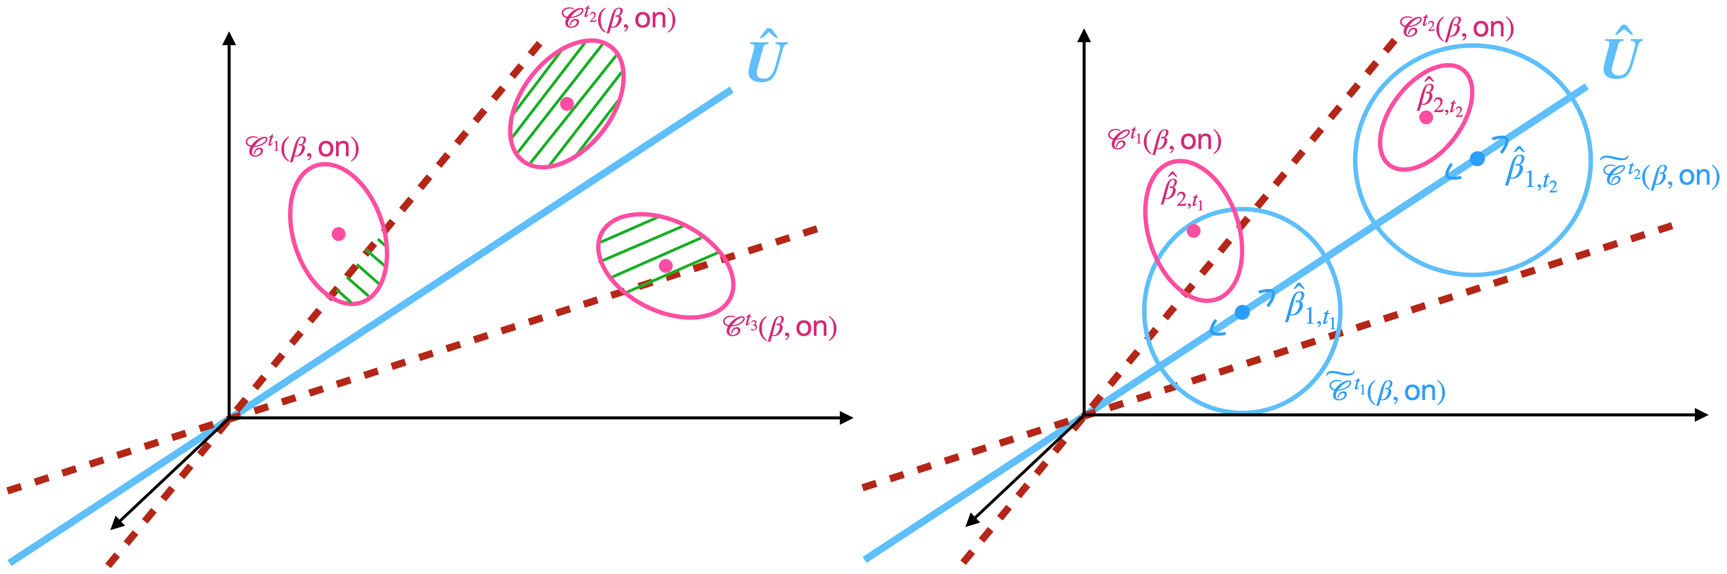
\includegraphics[width=\linewidth]{figures/ch03/imgs/figures/local-proball-ucb.png}
    \caption{\textbf{Left:} Geometric interpretations of \aigen{Algorithm~\ref{alg:local-ucb}}. Showing $\gC^{t}_{\on}(\bbeta) \cap \gC^{t}_{\off}(\bbeta)$ in green for three timepoints $t=t_1, t_2, t_3$. The dotted lines delineate the subspace confidence set. \textbf{Right:} Geometric interpretation of \aigen{Algorithm~\ref{alg:proball-ucb}}. $\gC^{t_1}_{\on}(\bbeta) \not\subset \widetilde \gC^{t_1}_{\off}(\bbeta)$, so we continue to use projections; but by time $t_2,$ $\gC_{\on}^{t_2}(\bbeta) \subset \widetilde \gC_{\off}^{t_2}(\bbeta)$, so we stop using projections.}
    \label{fig:geometric-motivation}
     
\end{figure}
While \aigen{Algorithm~\ref{alg:local-ucb}} is minimax-optimal, it is not computationally efficient due to the non-convex constraint discussed in Section~\ref{sec:local-ucb}. We address this by introducing \aigen{Algorithm~\ref{alg:proball-ucb}}, a practical and computationally efficient algorithm. In this section, we first sketch the algorithm and then describe how it can be geometrically motivated as a relaxation of \aigen{Algorithm~\ref{alg:local-ucb}}.

\aigen{Algorithm~\ref{alg:proball-ucb}} works in the subspace estimated by \aigen{Algorithm~\ref{alg:sold}} until the online confidence set is small enough. The algorithm maintains a low-dimensional confidence set, a high-dimensional confidence set, and swaps between them to achieve acceleration. Once the cumulative error of using the low-dimensional confidence set ($\approx \Delta_{\off}T$ in \aigen{Algorithm~\ref{alg:proball-ucb}}) exceeds the cumulative error of using the high-dimensional confidence set ($\approx d_A\sqrt{T}$), we stop using the former. This is instantiated with LinUCB, but the same idea can be immediately applied to other algorithms like SupLinUCB or Bayesian algorithms like Thompson sampling. 

% \begin{figure}
%     \centering
%     \includegraphics[width=0.5\linewidth]{figures/ch03/imgs/figures/proball-ucb.png}
%     \caption{Left: Geometric interpretations of \aigen{Algorithm~\ref{alg:local-ucb}}. Showing $\gC^{t}_{\on}(\bbeta) \cap \gC^{t}_{\off}(\bbeta)$ in green for three timepoints $t=t_1, t_2, t_3$. The dotted lines delineate the subspace confidence set. Right: Geometric interpretation of \aigen{Algorithm~\ref{alg:proball-ucb}}. $\gC^{t_1}_{\on}(\bbeta) \not\subset \widetilde \gC^{t_1}_{\off}(\bbeta)$, so we continue to use projections; but by time $t_2,$ $\gC_{\on}^{t_2}(\bbeta) \subset \widetilde \gC_{\off}^{t_2}(\bbeta)$, so we stop using projections.}
%     \label{fig:enter-label}
% \end{figure}

We geometrically motivate our update rule here as a relaxation of \aigen{Algorithm~\ref{alg:local-ucb}}, and illustrate it in Figure~\ref{fig:geometric-motivation}, like in Section~\ref{sec:local-ucb}. 
% Unlike \aigen{Algorithm~\ref{alg:local-ucb}}, we do not use a union of $d_K$-dimensional ellipsoids to construct the offline confidence set. We instead consider the subspace estimated by \aigen{Algorithm~\ref{alg:sold}}, compute a point estimate for $\beta_\star$ within the subspace, and construct a ball that contains the \aigen{Algorithm~\ref{alg:local-ucb}} offline confidence set. Using a ball will make optimism more tractable, and we call this offline confidence set $\widetilde \gC^t_{\off}(\bbeta)$. We use the usual $d_A$-dimensional confidence ellipsoid as the online confidence set, calling it $\gC^t_{\on}(\bbeta)$ again. Instead of actually intersecting the offline and online confidence sets, we relax the optimism further. We aim to be optimistic over the offline confidence ball until the online confidence set is inside it. Finally, to compute whether one set is inside the other, we use a proxy condition which roughly demands that $\Delta_{\off}T > d_A\sqrt{T}$.
We go through three stages of simplification over \aigen{Algorithm~\ref{alg:local-ucb}}, which suprisingly only leads to a minor degradation in provable guarantees.
 
\begin{itemize}  
\item Cruder offline confidence sets are used. We take the subspace estimated by \aigen{Algorithm~\ref{alg:sold}}, compute a point estimate for $\beta_\star$ within the subspace, and construct a ball that contains the \aigen{Algorithm~\ref{alg:local-ucb}} offline confidence set. The online confidence set is still the standard $d_A$-dimensional ellipsoid.
\item We wait for the offline confidence ball to contain the online confidence set, instead of taking intersections.
\item We use a computable proxy for this subset condition instead of explicitly checking it.
\end{itemize}
 
% \cknote{Make more conversational.} To geometrically motivate our update rule like in Section~\ref{sec:local-ucb}, we consider the $d_K$-dimensional confidence ellipsoid $\gC^t(\bbeta, \hat \BU)$ of $\bbeta$ \textit{inside} subspace $\hat \BU^\top$. First, since $\|\hat \BU \hat \BU^\top - \BU_\star \BU_\star^\top\|_2 \leq \Delta_{\off}$, we can show that a crude bound for $\phi(x,a)^\top \bbeta_\star$ is $\max_{\bbeta \in \gC^t(\bbeta, \hat \BU)} \phi(x,a)^\top \bbeta + \Delta_{\off}$. This corresponds to  optimism over a crude confidence ball $\widetilde \gC^t_{\off}(\bbeta)$ of radius $\Delta_{\off}$ around $\gC^t(\beta, \hat \BU)$. Second, instead of being optimistic over the intersection of this ball with our usual $d_A$-dimensional confidence ellipsoid $\gC^t_{\on}(\bbeta)$, we merely wait for $\gC^t_{\on}(\bbeta)$ to be inside $\widetilde \gC^t_{\off}(\bbeta)$. Finally, instead of actually checking whether $\gC^t_{\on}(\bbeta)$ is inside $\widetilde \gC^t_{\off}(\bbeta)$, we use a proxy condition that roughly demands $\Delta_{\off}T > d_A\sqrt{T}$. Here, $d_A\sqrt{T}$ represents the "cumulative size" of the ellipsoid across timesteps $t$, while $\Delta_{\off}T$ represents the "cumulative size" of the ball. This is illustrated in Figure \ref{fig:enter-label}.



\begin{algorithm}[htbp!]
\centering
	\caption{\aigen{Projected Confidence-Ball Optimistic Linear Bandit}}
    \label{alg:proball-ucb}
	\begin{algorithmic}[1]
	    \STATE \textbf{Input:} Projection matrix $\hat \BU \hat \BU^\top$, confidence bound $\Delta_{\off}$. Hyperparameters $\alpha_{1,t}, \alpha_{2,t}, \tau, \tau'$.
        \STATE \textbf{Initialize} $\BV_1 \gets I$, $\bb_{1} \gets 0$, $\BC_t \gets 0$
        \FOR{$t= 1,\dots T$}
            \IF{$ \Delta_{\off} \tau\sqrt{t} + \Delta_{\off}\tau'\sqrt{{d_K}\textstyle{\sum}_{s=1}^t \kappa_s^2/t} \leq d_A$}
            \STATE \textbf{Compute} $\hat \bbeta_{1,t} \gets \hat \BU (\hat \BU^\top \BV_{t} \hat \BU)^{-1} \hat \BU^\top \bb_t$
            \STATE \textbf{Play} $a_t \gets \arg\max_{a} \phi(x_t, a)^\top \hat \BU \hat \BU^\top \hat \bbeta_{1,t} 
            + \alpha_{1,t}\Vert\phi(x_t, a)^\top \hat \BU\Vert_{(\hat \BU^\top \BV_t \hat \BU)^{-1}}$
            \ELSE 
            \STATE \textbf{Compute} $\hat \bbeta_{2,t} \gets \BV_{t}^{-1} \bb_t$
            \STATE \textbf{Play} $a_t \gets \arg\max_{a} \phi(x_t, a)^\top \hat \bbeta_{2,t} + \alpha_{2,t}\left\Vert\phi(x_t, a)\right\Vert_{\BV_t^{-1}}$
            \ENDIF
            \STATE \textbf{Observe} reward $r_t$ and update $\bb_{t+1} \gets \bb_t + \phi(x_t, a)r_t$, $\BV_{t+1} \gets \BV_t + \phi(x_t, a)\phi(x_t, a)^\top$
            \STATE \textbf{Update} $\BC_{t+1} \gets \BC_t + \hat \BU^\top \phi(x_t, a_t)\phi(x_t, a_t)^\top $, $\kappa_{t+1} \gets \|\BC_{t+1}\|_{(\hat \BU^\top \BV_{t+1} \hat \BU)^{-1}}$
        \ENDFOR
	\end{algorithmic}
\end{algorithm}
As a final note before the regret bound, there is a technical challenge with analyzing \aigen{Algorithm~\ref{alg:proball-ucb}}. Since $\hat \bbeta_{1,t}$ lies in $\hat \BU$ but $\bbeta_\star$ might not, the $d_K$-dimensional confidence ellipsoid bound no longer applies. We therefore prove our own confidence ellipsoid bound in Lemma~\ref{lem:self-norm-conc}, to bypass this issue.
 
\begin{restatable}[Regret for \aigen{Algorithm~\ref{alg:proball-ucb}}]{theorem}{ProBALLUCB}\label{thm:proball-ucb}
    Let $\alpha_{1,t} = R\sqrt{\mu} + \tau'R\Delta_{\off}\kappa_t + CR\sqrt{d_K\log(T/\delta)}$ and let $\alpha_{2,t} = R\sqrt{\mu} + CR\sqrt{d_A\log(T/\delta)}$. Let $S$ be the first timestep when Algorithm~\ref{alg:proball-ucb} does not play Line 6 and let $S=T$ if no such timestep exists. For $\tau = \tau' = 1$ we have that 
    \begin{align*}
     \Reg_T &= \textstyle{\widetilde O\left(\min\left(\Reg_{on,T}, \Reg_{hyb, T}\right)\right)}.
\end{align*}
where $\Reg_{on,T} = Rd_A\sqrt{T}$ and $\Reg_{hyb,T} = Rd_K\sqrt{T}\left(1 + \frac{1}{\lambda_A^3\lambda_{\theta}}\left(\sqrt{\frac{d_AT}{d_KN}} + \sqrt{\frac{d_A}{SN}\sum_{t=1}^{S}\kappa_t^2}\right)\right)$
In the worst case, $\kappa_t = O(t)$ and so $\frac{1}{S}\sum_{t=1}^{S}\kappa_t^2 = O(T^2)$, but if all features $\phi(x_t, a_t)$ lie in the span of $\hat \BU$ for $t \leq S$, then $\frac{1}{S}\sum_{t=1}^{S}\kappa_t^2 = O(T)$.
\end{restatable}
While the regret bound looks weaker in the worst case, we emphasize that the "good case" in Theorem~\ref{thm:proball-ucb} is quite common. As an illustrative example, if the feature set $\gF_t = \{\phi(x_t,a) \mid a \in \gA\}$ is an $\ell_2$ ball, then the maximization problem in Step 6 will always choose $a_t$ with $\phi(x_t, a_t)$ in the span of $\hat \BU$. This can also approximately hold if the features are roughly isotropic or close to the span of $\hat \BU$.

 
\section{Experiments}
\label{sec:experiments}
 

% \begin{figure*}[tb!]
%     \centering
%     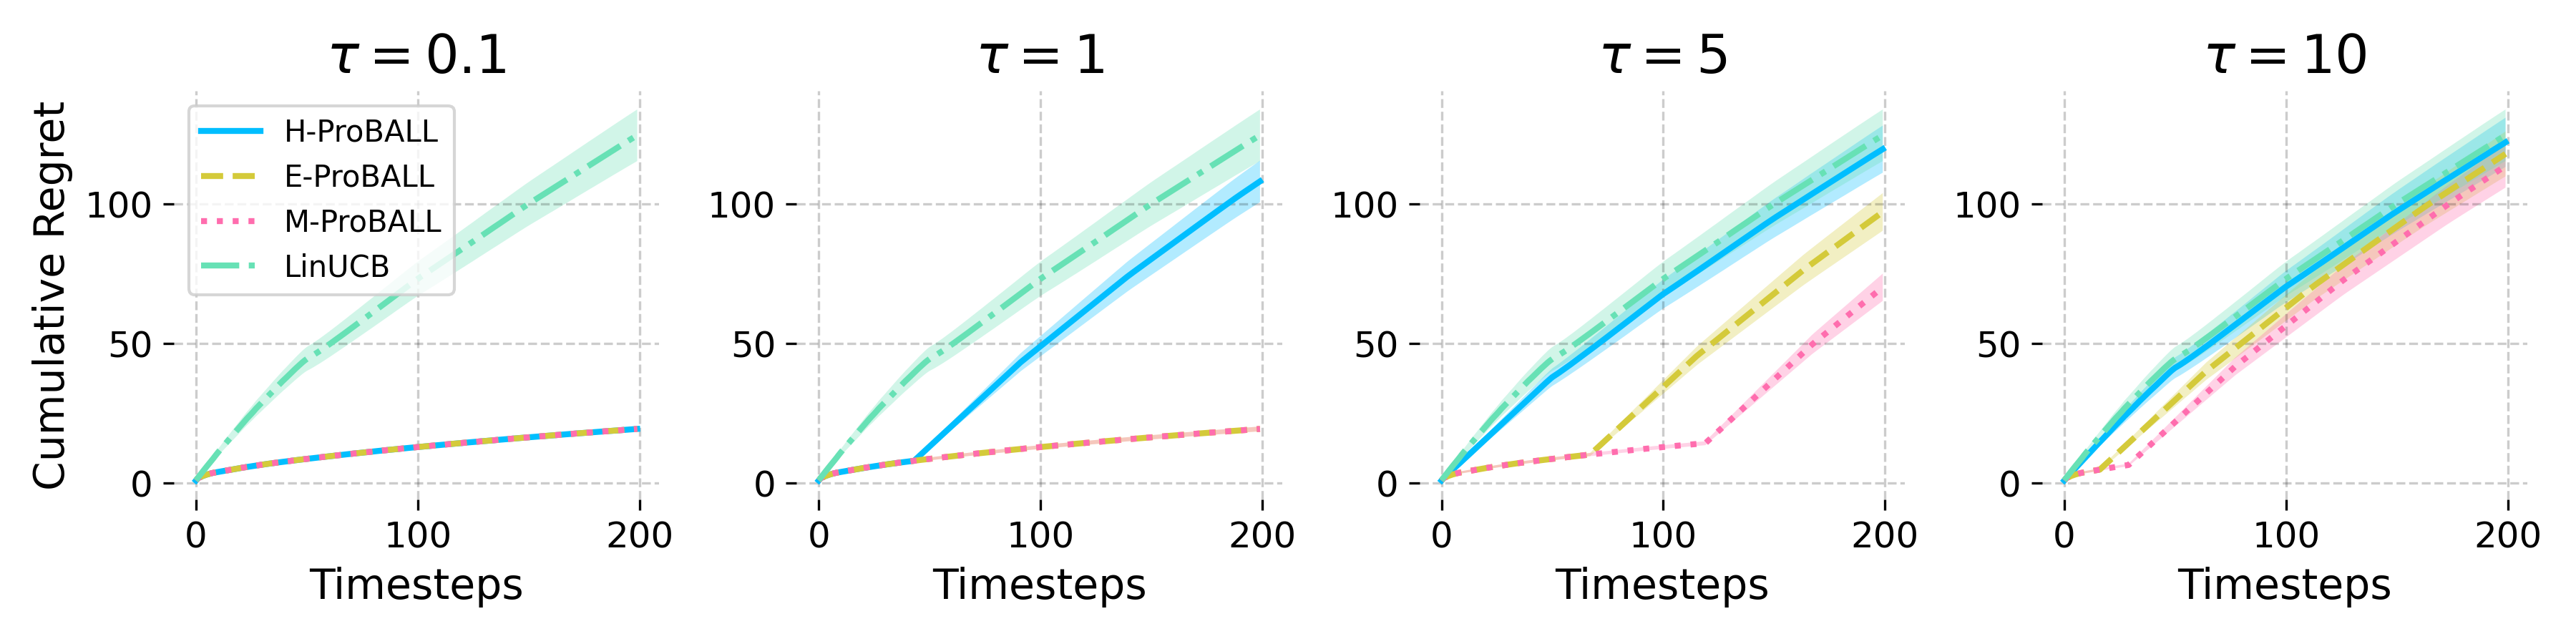
\includegraphics[width=\textwidth]{figures/ch03/imgs/sims/bayes_regret_sims.png}
%     \caption{Comparison of \aigen{Algorithm~\ref{alg:proball-ucb}} with LinUCB, for different choices of $\tau$ and confidence bound constructions. All variants perform no worse than LinUCB, with martingale Bernstein performing the best. The shaded area depicts $1$-standard error confidence intervals over $30$ trials.}
%     \label{fig:regret-sims}
%      
% \end{figure*}

\begin{figure*}[htbp!]
    \centering
    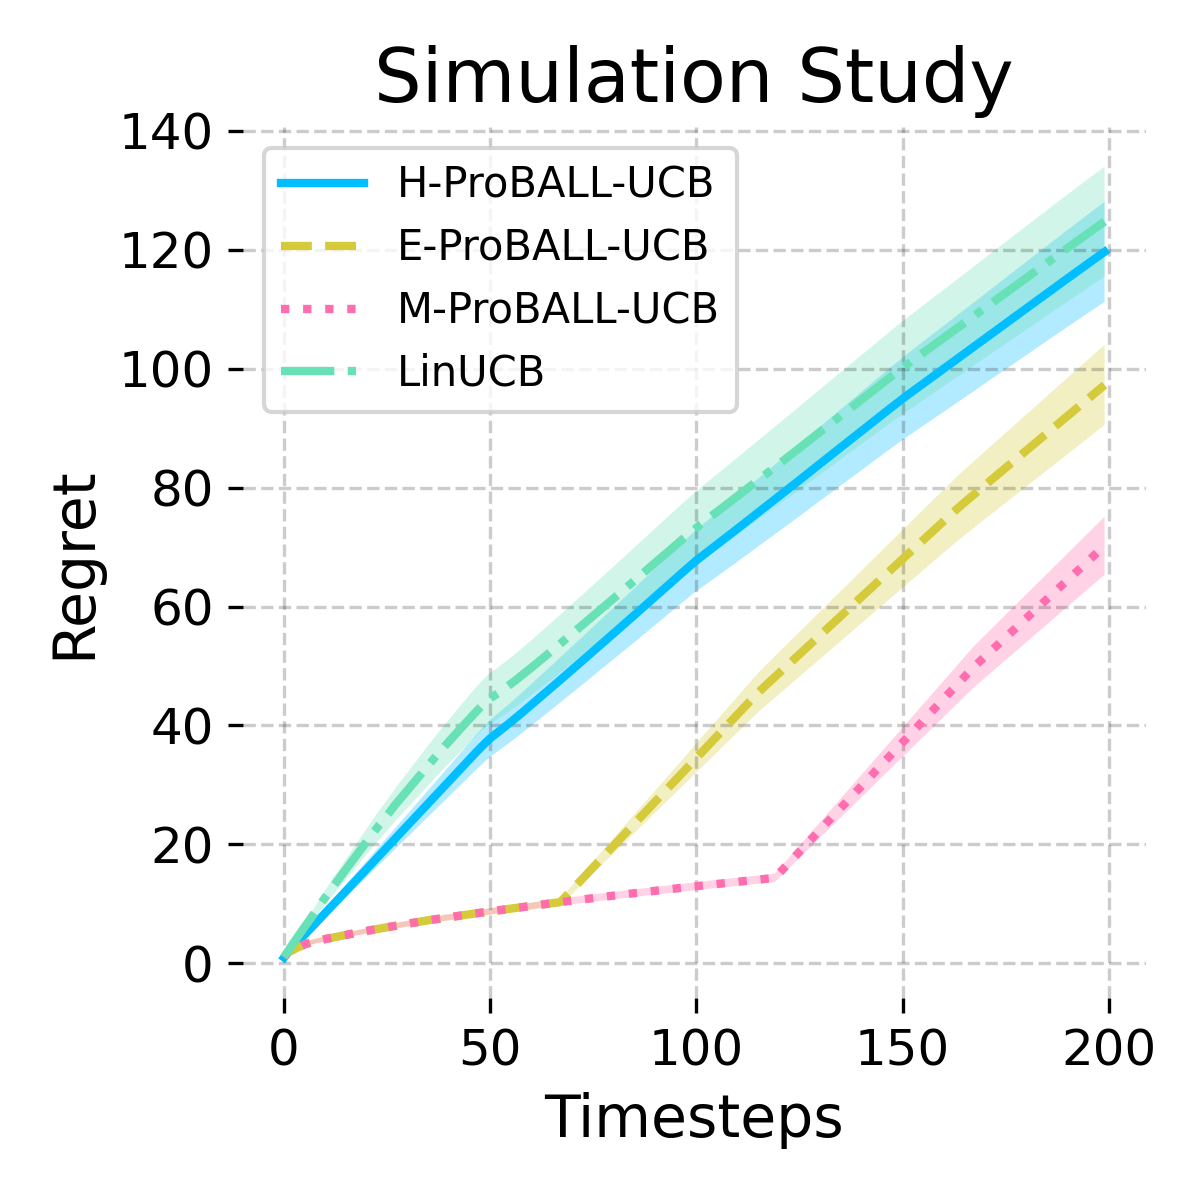
\includegraphics[width=0.24\textwidth]{figures/ch03/imgs/sims/solobayes_regret_sims.png}
    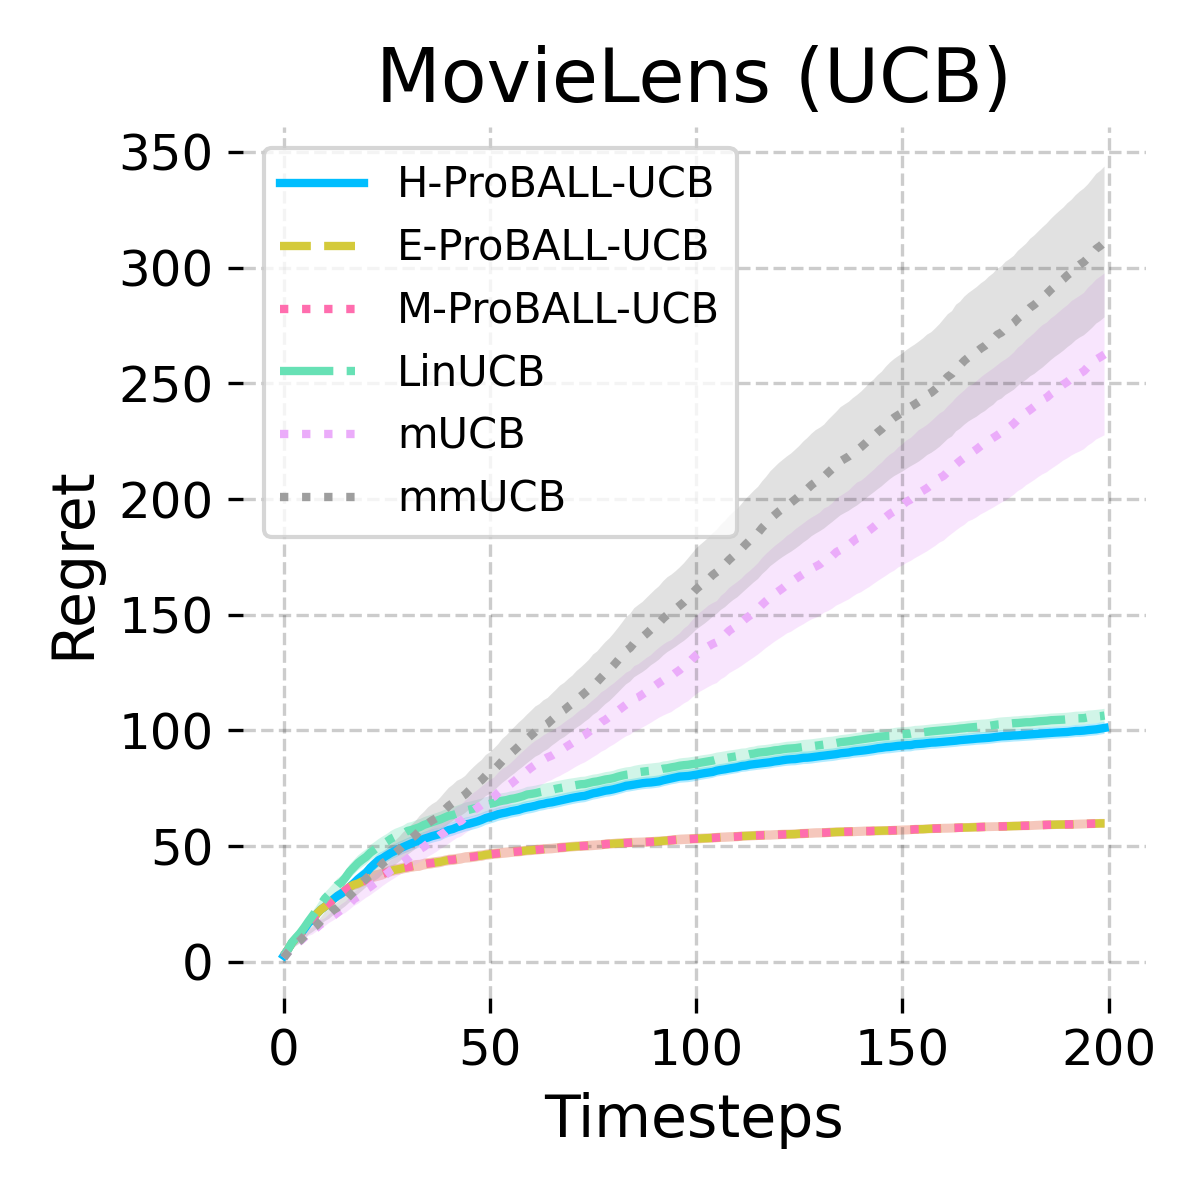
\includegraphics[width=0.24\textwidth]{figures/ch03/imgs/movies/solo_bayes_regret_ucb_movies.png}
    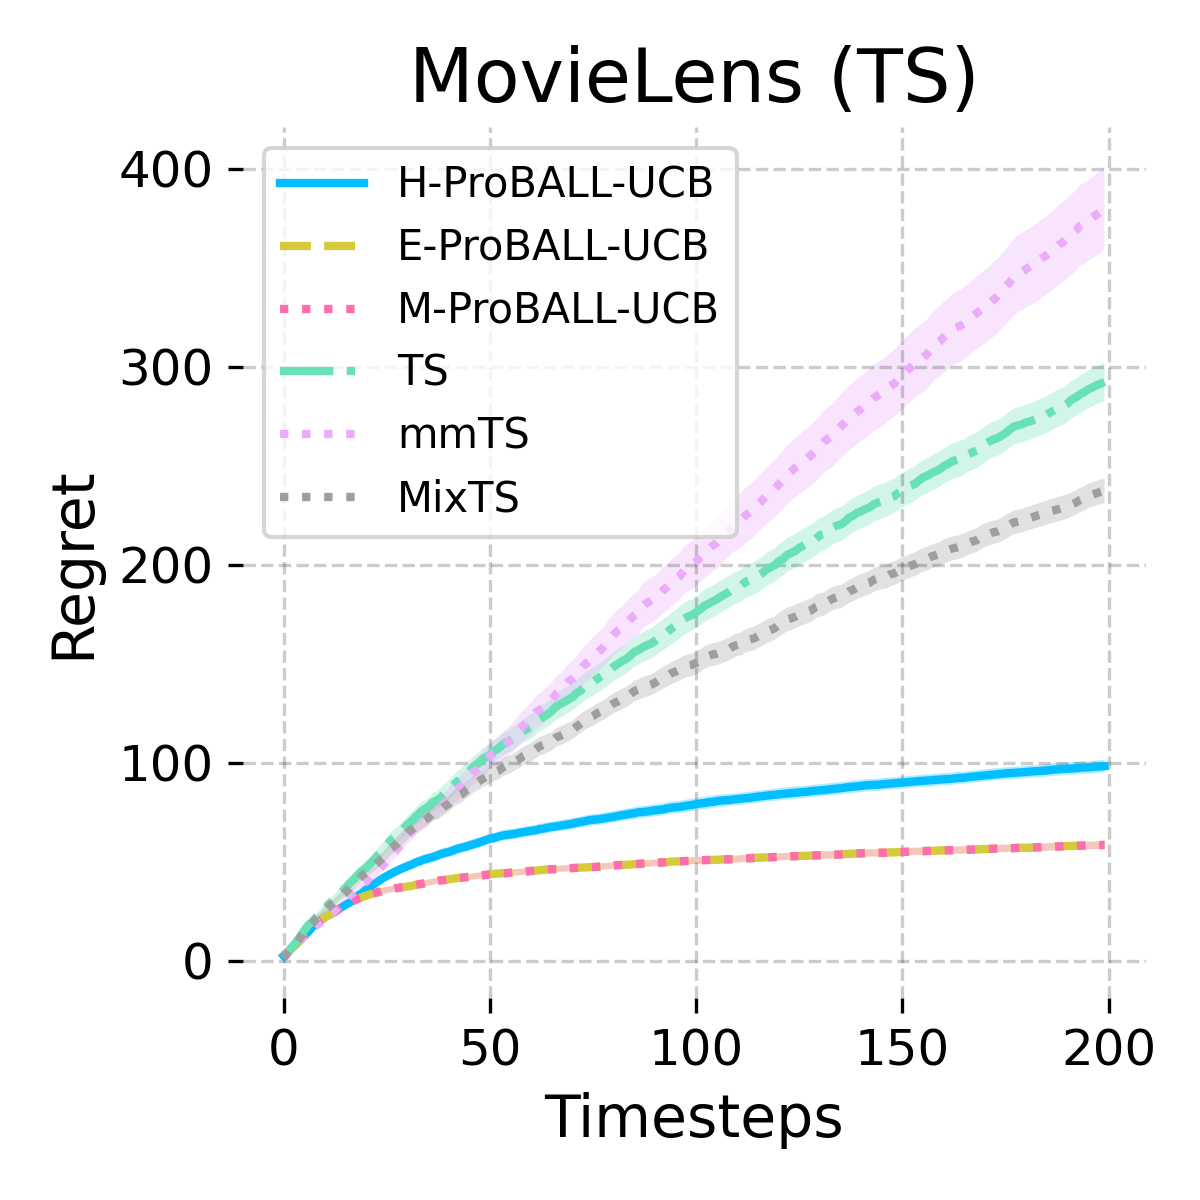
\includegraphics[width=0.24\textwidth]{figures/ch03/imgs/movies/solo_bayes_regret_ts_movies.png}
    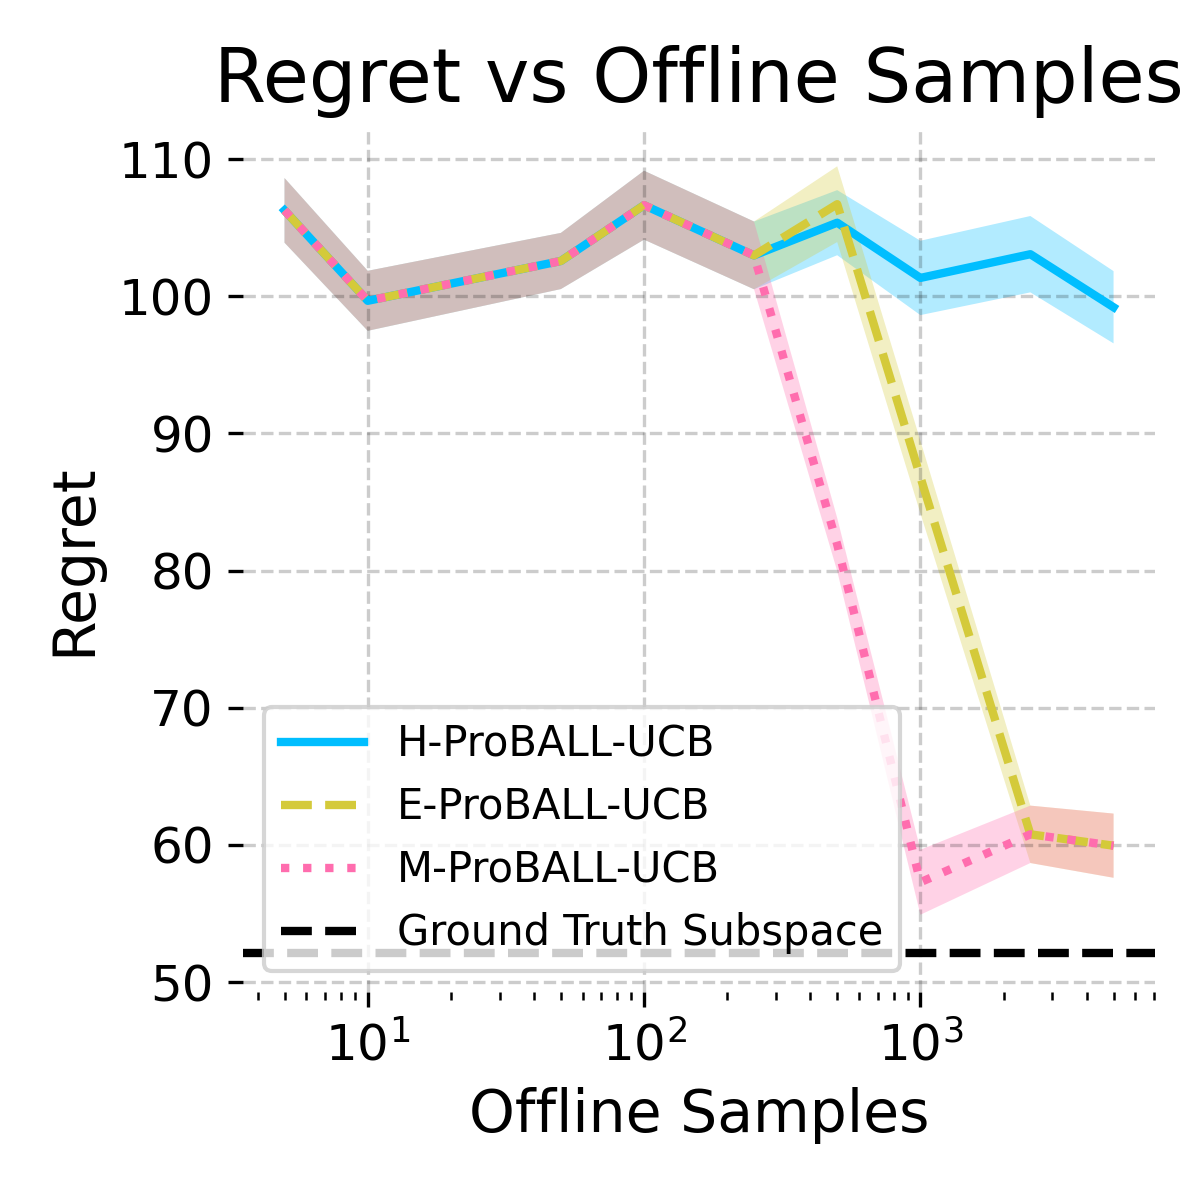
\includegraphics[width=0.24\textwidth]{figures/ch03/imgs/movies/solo_bayes_subspace_sample_comp_movies.png}
    \caption{Left to Right. \textbf{First:} Simulation study comparison of \aigen{Algorithm~\ref{alg:proball-ucb}} against LinUCB for $\tau=5$. \textbf{Second/Third:} Comparison of \aigen{Algorithm~\ref{alg:proball-ucb}} initialized with \aigen{Algorithm~\ref{alg:sold}} against $\{$LinUCB, mUCB, and mmUCB, TS, mmTS, and MixTS$\}$, for $\tau=0.1$ and various confidence bound constructions. \aigen{Algorithm~\ref{alg:proball-ucb}} outperforms all other algorithms, and approaches the performance of LinUCB when Hoeffding confidence sets are used. \textbf{Fourth}: \aigen{Algorithm~\ref{alg:proball-ucb}} regret on MovieLens against offline samples used in \aigen{Algorithm~\ref{alg:sold}}, compared to LinUCB on ground-truth low-dimensional features. Here, $\tau=0.1,T=200$. As the number of offline samples increases, \aigen{Algorithm~\ref{alg:sold}} recovers a low-rank subspace almost as good as ground-truth. The shaded area in each sub-figure depicts $1$-s.e. confidence intervals over $30$ trials with fresh $\btheta$, accounting for the variation in frequentist regret for changing $\btheta$.}
    \label{fig:regret-movies}
     
\end{figure*}

We now establish the practical efficacy of \aigen{Algorithm~\ref{alg:sold}} and \aigen{Algorithm~\ref{alg:proball-ucb}} for linear latent contextual bandits through a series of numerical experiments. We perform a simulation study and a demonstration using real-life data. While specific details of the experiments and many ablation studies are in Appendix~\ref{app:experiments}, we sketch our experiments and discuss key observations in this section.

 
In all experiments, we obtain confidence bounds $\Delta_{\off}$ using three different concentration inequalities -- (1) Hoeffding as in Proposition \ref{prop:conf-bound-d} (H-ProBALL), (2) empirical Bernstein as in Proposition \ref{prop:conf-bound-bbm} (E-ProBALL), and (3) the martingale Bernstein concentration inequalities of \cite{ian2023betting} (M-ProBALL). We use a simpler expression for $\Delta_{\off}$, set $\tau'=0$, and choose a suitable value of the hyperparameter $\tau$ to adjust for overly conservative $\Delta_{\off}$\footnote{Namely, we set $\Delta_D=0$ in $\Delta_{\off}$. Also, Lemma~\ref{lem:self-norm-conc} and~
some thought reveal that choosing $\tau'=0$ recovers the "good" version of \aigen{Algorithm~\ref{alg:proball-ucb}} guarantees, if features are isotropic enough.}. We later vary $\tau$ in ablation experiments to demonstrate that our results are not a consequence of our choice of hyperparameters. Finally, for the MovieLens experiments, we additionally design a natural Thompson sampling version of \aigen{Algorithm~\ref{alg:proball-ucb}} to highlight the applicability of the ProBALL idea called \aigen{projected confidence-ball Thompson sampling (Algorithm~\ref{alg:proball-ts})} in Appendix \ref{app:algorithms}. All experiments for \aigen{projected confidence-ball Thompson sampling (Algorithm~\ref{alg:proball-ts})} are in Appendix~\ref{app:proball-ts}.


\textbf{Simulation study.} We first perform a simulation study on a latent linear bandit with $d_A=50$ and $d_K=2$, with $5000$ trajectories generated offline. Further details are provided in Appendix~\ref{app:experiments}, and the results are presented in Figure \ref{fig:regret-movies}. Note that \aigen{Algorithm~\ref{alg:proball-ucb}} performs no worse than LinUCB, no matter what we choose for $\tau$ and $\Delta_{\off}$. However, we see a clear benefit from using tighter confidence bounds -- as $\Delta_{\off}$ gets smaller, Algorithm~\ref{alg:proball-ucb} chooses to utilize the projected estimate $\hat\bbeta_{1,t}$ more often, resulting in better performance. Note that the kinks in the regret curves correspond to points where Algorithm~\ref{alg:proball-ucb} switches over to the higher dimensional optimism in step 7.

 
\textbf{MovieLens dataset.} In line with \cite{hong2020latent}, we assess the performance of our algorithms on real data using the MovieLens dataset. Like them, we filter the dataset to include only movies rated by at least $200$ users and vice versa, and apply probabilistic matrix factorization (PMF) to the rating matrix to generate ground truth user preferences for online experiments. Applying PMF gives $d_K = 18$ and we choose $d_A = 200$, generating 5000 trajectories offline. For baselines, we reproduce the methods of \cite{hong2020latent, hong2022thompsonsamplingmixtureprior} and implement LinUCB with canonical hyperparameter choices.

 
We initialize \aigen{Algorithm~\ref{alg:proball-ucb}} with a subspace estimated with an unregularized variant of \aigen{Algorithm~\ref{alg:sold}} (see Appendix \ref{app:algorithms}) that uses pseudo-inverses instead of inverses. This is due to difficulties in finding an appropriate regularization parameter for this large, noisy, and high-dimensional dataset. Figure \ref{fig:regret-movies} depicts the result of this experiment. Once again, \aigen{Algorithm~\ref{alg:proball-ucb}} performs no worse than LinUCB, no matter what we choose for $\tau$ and $\Delta_{\off}$, and the benefit of using tighter confidence bounds remains. With $\tau=0.5$, \aigen{Algorithm~\ref{alg:proball-ucb}} with martingale Bernstein confidence bands stops using the projected estimates at around timestep $70$, but still continues to outperform LinUCB. Although mUCB and mmUCB perform slightly better than \aigen{Algorithm~\ref{alg:proball-ucb}} and LinUCB at the beginning, the model misspecification incurred by discretizing the features into $d_K$ clusters ensures that it typically suffers linear regret in this scenario. The lower initial performance of \aigen{Algorithm~\ref{alg:proball-ucb}} and Lin-UCB is a consequence of their higher initial exploration.

 
\textbf{Ablation study.} While the end-to-end performance of \aigen{Algorithm~\ref{alg:proball-ucb}} significantly improves over existing algorithms, we also address questions about various components of our method in Appendix \ref{app:experiments}. First, we study the effect of varying the hyperparameter $\tau$ and note that our method stably outperforms existing methods at all reasonable values of $\tau$. Second, we compare different combinations of algorithms in our figures above, side by side. Finally, we evaluate the effect of offline data by plotting the online regret against the number of offline samples. 

 
\section{How General Are Latent Bandits?}\label{sec:de-finetti}

While have established that latent bandits are a powerful framework for accounting for uncertainty in reward models, the extent of their generality is unclear. Are there other stateless decision processes that generalize over latent bandits? We cap off our contributions by establishing the generality of latent bandits. In this section, we show a de Finetti theorem for decision processes, demonstrating that \textit{every} "coherent" and "exchangeable" stateless (contextual) decision process is a latent (contextual) bandit. We first define a stateless decision process at a high level of generality.\footnote{\cite{liu2023definition} work with a much more restrictive notion of a generalized bandit and use the original de Finetti theorem in~some of their lemmas. See Appendix~\ref{subapp:de-finetti-disc} for a discussion.} 
\begin{definition}
    A \textit{stateless decision process} (SDP) with action set $\gA$ is a probability space $(\Omega, \gG, \prob)$ with a family of random maps $\gF_H: \Omega \to (\gA^H \to \Real^H)$ for $H \in \N \cup \{\infty \}$.
\end{definition}
That is, given a sequence of actions $(a_1, \dots a_H)$, an SDP generates a random sequence of rewards $(Y_1, \dots Y_H)$. As such, we abuse notation to denote by $\gF_H(a_1, \dots a_H)$ the random variable $\omega \mapsto \gF_H(\omega)(a_1, \dots a_H)$. Without any coherence between $\gF_H$ across $H$, a stateless process can behave arbitrarily for different horizons $H$. We present a natural coherence condition below, essentially requiring that a given action sequence should produce consistent rewards.
%  
\begin{definition}
\label{defn:coherence}
A stateless decision process is \textit{coherent} if for any $h \leq k \leq H, H' \in \N \cup \{\infty\}$ and for any two action sequences $\tau, \tau'$ of lengths $H$ and $H'$ sharing the same actions $(a_h, \dots a_k)$ from index $h$ to $k$, with $\gF_{H}(\tau) = (Y_1, \dots Y_{H})$ and $\gF_{H'}(\tau') = (Y_1', \dots Y_{H'}')$, we have $(Y_h, \dots Y_k) = (Y_h', \dots Y_k')$, viewed as functions of $\Omega$.
\end{definition}
It is natural to require equality in value and not just in distribution, since after taking an extra action, the \textit{values} of past rewards stay the same, not just their \textit{distribution}. For example, if we pull 10 different jackpot levers and then pull a new one, the previous 10 outcomes stay the same in value, not just in distribution. We also give a natural definition for exchangeability of a stateless decision process -- namely that exchanging any two rewards should lead to the distribution obtained by exchanging the corresponding actions.
\begin{definition}
    A stateless decision process is \textit{exchangeable} if for any permutation $\pi: [H] \to [H]$ and $\gF_H(a_1, \dots a_H) = (Y_1, \dots Y_H)$, we have $\gF_h(a_{\pi(1)}, \dots a_{\pi(H)}) \sim (Y_{\pi(1)}, \dots Y_{\pi(H)})$.
\end{definition}
Finally, a latent bandit is an SDP that behaves like a bandit \textit{conditioned} on a random latent state $F$ that determines the reward distribution. As $F$ determines a distribution, it is a random measure-valued function on $\gA$.


\begin{definition}
    A latent bandit is a stateless decision process equipped with a random measure-valued function $F: \Omega \to (\gA \to \gP(\Real))$ so that for any $H$ and action sequence $(a_1, \dots a_H)$, the rewards $(Y_1, \dots Y_H) := \gF_H(a_1, \dots a_H)$ are independent conditioned on $F$. Moreover, the conditional distribution $\gL[Y_h \mid F] = F(a_h)$ for all $h\leq H$.\footnote{We abuse notation twice here. First, we write $F(a_h) := (\omega \mapsto F(\omega)(a_h))$. Second, as the regular conditional distribution $\gL[Y_h \mid F]$ is a kernel that maps from $\Omega \times \gB \to \Real$, we view $F(a_h)$ as its curried map $(\omega, B) \mapsto F(a_h)(\omega)(B)$. A discussion of issues (measurability and well-definedness) is in Appendix \ref{app:definetti}.}
\end{definition}
While exchangeability and coherence are reasonable conditions on an SDP and are clearly satisfied by latent bandits, it is a-priori unclear if they are sufficient to ensure that the SDP is a latent bandit. As only exchanging rewards from the \textit{same action} preserves the distribution, standard de Finetti proof ideas do not immediately apply. After all, it is possible that an SDP could be cleverly designed to choose rewards adaptively across time and satisfy these properties. Reassuringly, no such counterexamples exist, guaranteed by the following theorem.
\begin{restatable}[De Finetti Theorem for Stateless Decision Processes]{theorem}{DeFinetti}\label{thm:definetti}
    Every exchangeable and coherent stateless decision process is a latent bandit.
\end{restatable}
We show in Lemma~\ref{lem:coh-equality} in Appendix~\ref{app:additional-lemmas} that coherence is not a consequence of exchangeability -- it is a necessary condition for being a latent bandit. Finally, we analogously consider contexts and define "transition-agnostic contextual decision processes" (TACDPs) in Appendix~\ref{app:definetti}. We define coherence and coherence and exchangeability for TACDPs, and define latent \textit{contextual} bandits by simply replacing $\gA$ with $\gX \times \gA$ in the definitions above. We then show an analogous de Finetti theorem, as a corollary of our proof of Theorem~\ref{thm:definetti}. See Appendix \ref{app:tacdps} for more details.
% Finally, we analogously consider contexts and define transition-agnostic contextual decision processes (TACDPs) in Appendix~\ref{app:definetti}. These are transition-agnostic in the sense that the process only carries the data of how rewards are generated from given sequences of contexts and actions, while the context transitions themselves may be generated by a different process. It is natural to isolate away context dynamics for processes like stochastic contextual bandits, in which actions do not affect the context transitions -- in contrast to transition-aware definitions in \cite{jiang2016contextual}. A formal definition is in Appendix \cknote{cite}, where we analogously define coherence and exchangeability for TACDPs and define latent \textit{contextual} bandits by simply replacing $\gA$ with $\gX \times \gA$ in the definitions above. We then show an analogous de Finetti theorem, as a corollary of our proof of Theorem~\ref{thm:definetti}. 
% Finally, we consider contexts and define contextual decision processes in a manner agnostic to context transitions. That is, the process only carries the data of how rewards are generated from given sequences of contexts and actions, while the context transitions themselves may be generated by a different process.
% \begin{definition}
%     A \textit{transition-agnostic contextual decision process} (TACDP) with action set $\gA$ and context set $\gX$ is a probability space $(\Omega, \gG, \prob)$ equipped with a family of random maps $\gF_H: \Omega \to ((\gX \times\gA)^H \to \Real^H)$ for $H \in \N$ as well as a map $\gF_\infty: \Omega \to ((\gX \times \gA)^\N \to \Real^\N)$.
% \end{definition}
% It is natural to isolate away context dynamics for processes like stochastic contextual bandits, in which actions do not affect the context transitions -- in contrast to transition-aware definitions in \cite{jiang2016contextual}. We can analogously define coherence and exchangeability for TACDPs and define latent \textit{contextual} bandits by simply replacing $\gA$ with $\gX \times \gA$ in the definitions above. We then show an analogous de Finetti theorem, as a corollary of our proof of Theorem~\ref{thm:definetti}. See Appendix \ref{app:definetti} for more details.

Finally, note that this section is faithful to the rest of this paper. A linear latent contextual bandit is a latent contextual bandit where the random measure-valued function $F: \Omega \to ((\gX \times \gA) \to \gP(\Real))$ is defined by setting $F(\omega)(x, a)$ to be the distribution given by $\phi(x,a)^\top \BU_\star\btheta(\omega) + \epsilon$, for any $\omega \in \Omega$ and $(x, a) \in (\gX \times \gA)$. 



 
\section{Discussion, Limitations and Further Work}
In this paper, we have addressed the problem of leveraging offline data to accelerate online learning in linear latent bandits. Our work has a few limitations. First, while \aigen{Algorithm~\ref{alg:proball-ucb}} is practical and computationally efficient, it has a slightly weaker worse-case guarantee than \aigen{Algorithm~\ref{alg:local-ucb}}. Second, when the data is noisy, it can be hard to tune the regularization $\mu$. We use a pseudoinverse-based version of \aigen{Algorithm~\ref{alg:sold}} in such a case (Appendix \ref{app:algorithms}), implemented in our code. Third, the offline uncertainty sets computed using $\Delta_{\off}$ can be overly conservative, and a discount hyperparameter $\tau$ must be fine-tuned online.

Despite these limitations, our work enjoys strong theoretical guarantees and convincing empirical performance. We hope that this method opens the door for developing other efficient and scalable algorithms for sequential decision-making with continuous latent states. One can use ideas presented in this paper to design similar algorithms for MDPs, linear MDPs, and RL or bandits with general function approximation. 

